\documentclass{article}

\usepackage[a4paper, margin=2cm]{geometry}
\usepackage[utf8]{inputenc}
\usepackage[T1]{fontenc}

\usepackage[czech]{babel}
\usepackage{fvextra}
\usepackage{csquotes}
\usepackage{parskip}

\usepackage{float}
\usepackage{graphicx}
\usepackage{amsmath}
\usepackage{siunitx}

\usepackage[hidelinks, unicode, pdfusetitle]{hyperref}

\graphicspath{{./images/}}

\title{35-2-X1 Oblázky}
\author{Benjamin Swart}

\begin{document}
\maketitle

\section{Odebírání řad}
\label{section:removal}

V zadání se píše, že můžeme odebírat dvojice nebo trojice kamínků. Jakékoliv přirozené číslo větší než jedna však můžeme vyjádřit jako součet dvojek a trojek, protože $4 = 2 + 2$, $5 = 2 + 3$, $6 = 2 + 2 + 2$, $7 = 2 + 2 + 3$, $8 = 2 + 2 + 2 + 2$, $9 = 2 + 2 + 2 + 3$ a podobně. To znamená, že můžeme sebrat jakoukoliv řadu kamínků stejné barvy o délce nejméně dvě.

Dá se snadno dokázat, že nikdy nedává smysl ze souvislé řady kamínků stejné barvy odebrat jen některé kamínky. Kratší řada nám bude bránit v odebírání jiných kamínků úplně stejně jako řada delší. Můžeme tedy bez obav odebírání kamínků v řadě odložit do okamžiku, kdy je odebereme všechny najednou.

\section{Zápis řešení}
\label{section:diagram}

Řešení řady kamínků můžeme zakreslit graficky. Řadu kamínků, kterou sebereme najednou, zakreslíme jako obdélník. Všechny podposloupnosti kamínků, které musíme vysbírat dříve, zakreslíme rekurzivně nad něj.

Dejme tomu, že máme takovéto kamínky:

\begin{figure}[H]
    \centering
    
\includegraphics[scale=1]{marbles.pdf}
\end{figure}

Pak můžeme jedno z řešení zakreslit takto:

\begin{figure}[H]
    \centering
    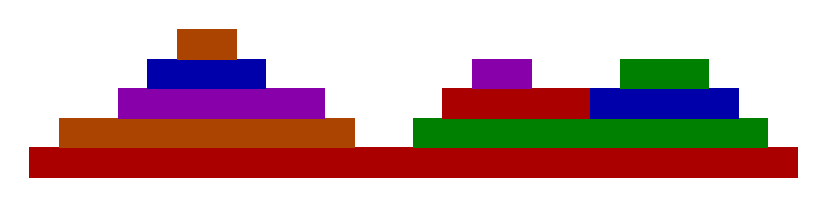
\includegraphics[scale=1]{solution.pdf}
\end{figure}

Podle jejich podoby v tomto diagramu můžeme odlišit dvě třídy řešitelných řad:

\subsection{Vrstva}

Vrstvou nazvu řadu dvou nebo více kamínků stejné barvy, která může být přerušena několika vyřešitelnými úseky oddělenými jednou nebo více kuličkami stejné barvy. Může vypadat například takto:

\begin{figure}[H]
    \centering
    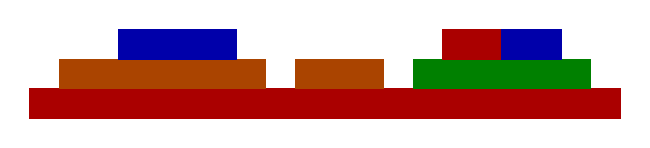
\includegraphics[scale=1]{layer.pdf}
\end{figure}

První a poslední kulička vrstvy musí mít nutně stejnou barvu.

Triviálním případem je čára, která se skládá jen z kuliček stejné barvy.

\subsection{Sekvence}

Sekvenci tvoří několik vyřešitelných úseků hned za sebou. Může vypadat například takto:

\begin{figure}[H]
    \centering
    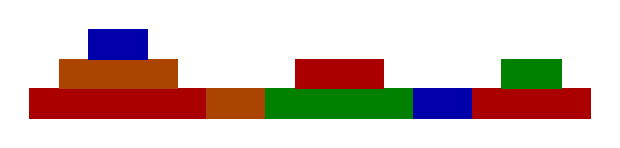
\includegraphics[scale=1]{sequence.pdf}
\end{figure}

\section{Hledání řešitelných řad}
\label{section:search}

Budeme postupně hledat všechny řešitelné úseky obsažené ve vstupu. Vytvoříme si matici $n \times n$, která bude mít na pozici $\left[i, j\right]$ jedničku právě tehdy, když bude interval kamínků $\left<i, j\right>$ řešitelný. Na začátku bude tato matice obsahovat samé nuly. Postupně do ní budeme doplňovat jedničky.

Nejprve do matice zapíšeme všechny řešitelné řady o délce 2, tj. dvojice kamínků stejné barvy. Poté do matice přidáme řešitelné řady o délce 3, 4, 5, 6, a tak dále až po řady o délce $n$. K nalezení intervalů o délce $m$ vždy využijeme již nalezené intervaly o délce $2$ až $m - 1$. Jak na to je popsáno v sekci \ref{section:composition}. Pokud nakonec najdeme řadu o délce $n$, neboli pokud bude na pozici $\left[1, n\right]$ jednička, tak je úloha řešitelná.

\section{Skládání řešitelných řad}
\label{section:composition}

Zbývá ještě popsat, jak najít řešitelné úseky o délce $m$ pomocí matice řešitelných úseků o délce $2$ až $m - 1$. K tomu nám poslouží klasifikace řešitelných řad popsaná v sekci \ref{section:diagram}. Jednoduše projdeme všechny možné intervaly $\left<i, j\right>$ o délce $m$ a ověříme, jestli splňují jednu z následujících podmínek:

\subsection{Sekvence}

Nejprve ověříme, jestli daná řada není sekvencí. To zjistíme tak, že ověříme, jestli je možné tuto řadu složit ze dvou menších řešitelných řad. Jinak řečeno, ověříme, zda existuje takové $k \in \left(i, j - 1\right)$, že $\left<i, k\right>$ a $\left<k + 1, j\right>$ jsou řešitelné intervaly. Tím najdeme nejen sekvence složené z dvou vrstev, ale sekvence delší, protože sekvenci o délce $s$ můžeme složit ze sekvence o délce $s - 1$ a posledního úseku.

\begin{figure}[H]
    \centering
    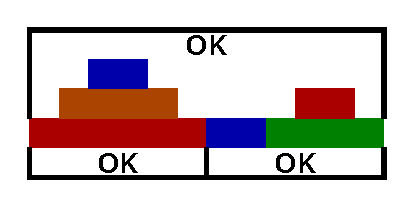
\includegraphics[scale=1]{solve-sequence.pdf}
\end{figure}

\subsection{Jednoduché vrstvy}

Poté ověříme, jestli se jedná o dvoukamínkovou vrstvu s jednou vnořenou řadou. Nejprve zkontrolujeme, zda mají $i$ a $j$ stejnou barvu, a poté zkontrolujeme, jestli je interval $\left<i + 1, j - 1\right>$ řešitelný.

\begin{figure}[H]
    \centering
    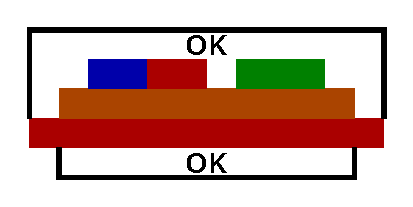
\includegraphics[scale=1]{solve-simple-layer.pdf}
\end{figure}

\subsection{Složité vrstvy}

Vrstvy s více kuličkami a vnořenými řadami složíme z menších. Nejprve ověříme, zda mají $i$ a $j$ stejnou barvu, a poté se pokusíme najít dva řešitelné intervaly s jednokamínkovým průnikem, ze kterých můžeme interval složit. Jinak řečeno, pokusíme se najít $k \in \left(i, j\right)$, kde $k$ má stejnou barvu jako $i$ a $j$ a kde jsou intervaly $\left<i, k\right>$ a $\left<k, j\right>$ řešitelné.

\begin{figure}[H]
    \centering
    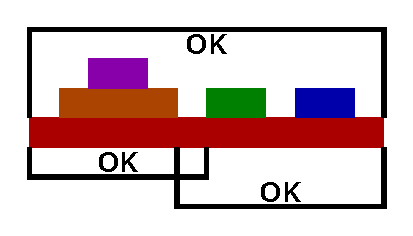
\includegraphics[scale=1]{solve-complex-layer.pdf}
\end{figure}

\begin{figure}[H]
    \centering
    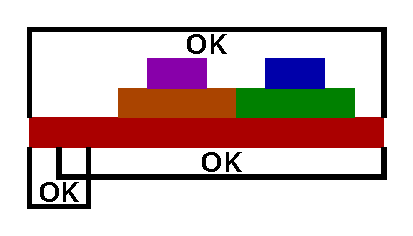
\includegraphics[scale=1]{solve-extended-layer.pdf}
\end{figure}

\section{Rekonstrukce strategie}

Pokud jsme ověřili existenci strategie, tak ji ještě musíme zrekonstruovat. K tomu můžeme použít naši matici. Pro interval $\left<1, n\right>$ znovu provedeme kontroly ze sekce \ref{section:composition}, čímž zjistíme, z jakých intervalů ho složíme. Totéž uděláme rekurzivně pro všechny dílčí intervaly. Z toho triviálně dopočítáme úplnou strategii.

\section{Analýza složitosti}
\label{section:analysis}

Postupně ověříme řešitelnost všech $\mathcal{O}\left(n^2\right)$ intervalů. Ve dvou ze tří provedených kontrol musíme ještě najít $k$, které má $\mathcal{O}\left(n\right)$ možných hodnot. Algoritmus tedy poběží v $\mathcal{O}\left(n^3\right)$. Největší datová struktura v paměti je matice $n \times n$. Paměťová složitost tedy bude $\mathcal{O}\left(n^2\right)$.

\end{document}
